\IEEEPARstart
{T}{he} second iteration of the design\dots

\subsection{Architecture \& Modularity}

\begin{figure}[h]
    \centering
    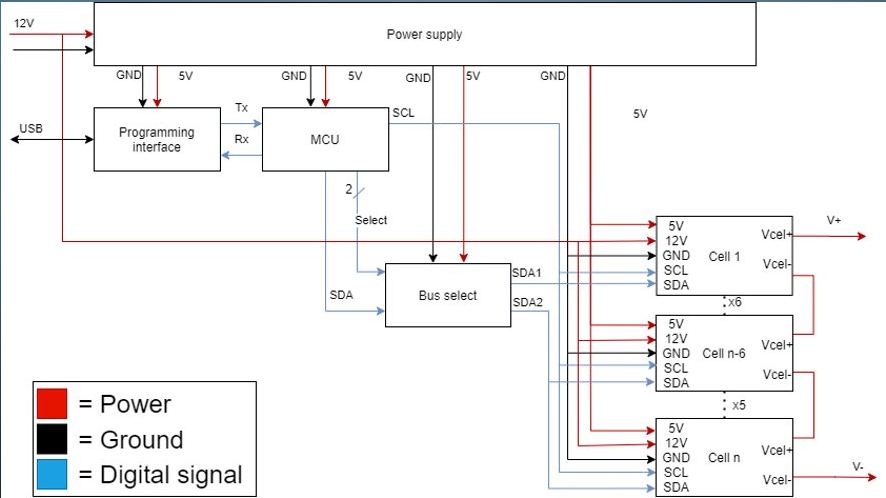
\includegraphics[scale=0.5]{architecture_2nd_iteration.png}
    \caption{Architecture block diagram of the 2nd iteration of the emulator.}
\end{figure}

The second iteration of the design is made modular, in order to be able to make 
possible working with multiple cells. This is done by implementing a model board
PCB and a cell board PCB. The model board houses 14 slots for cell boards to be 
connected to. This means that as many cells (up to 14) can be used (regardless 
of the slot position).

    \subsubsection{Model board}
    The model board consists of a 5 V power supply, the microcontroller, a USB 
    conneciton and 14 cell slots. The following is being transmitted at the
    cell slots:

    \begin{itemize}
        \item 12V from the external powersupply
        \item GND
        \item 5V from the on-board powersupply
        \item SDA
        \item SCL
    \end{itemize}

    \subsubsection{Cell board}
    The cell board has an isolated voltage barrier. The transmitted 12 V is 
    made into isolated 9 V using an isolated DC-DC converter, and the data is
    transmitted through the barrier using a bidirectional I2C isolator.

    On the other side of the barrier there is a voltage regulator that provides 
    the isolated 5 V needed to power everything, there is the digital potentiometer
    and the sinking and sourcing circuitry. There are also the address pins, which
    can be soldered in order to provide an address so that every cell board that 
    is connected to the model board can be distinguished. 

    \begin{figure}[h]
        \centering
        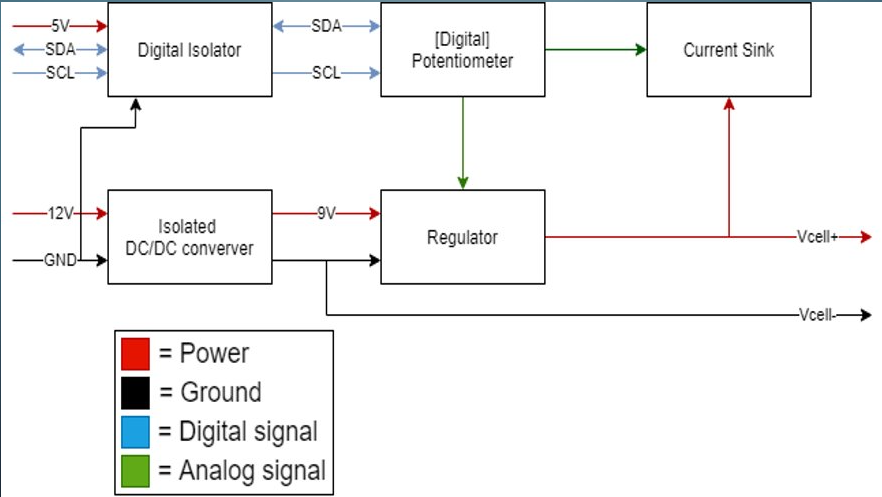
\includegraphics[scale=0.47]{architecture_single_cell.png}
        \caption{Architecture block diagram of the cell board.}
    \end{figure}

\subsection{Hardware}
Current sourcing sinking etc. text here.

\subsection{Software}
Software text here.

\begin{figure}[h]
    \centering
    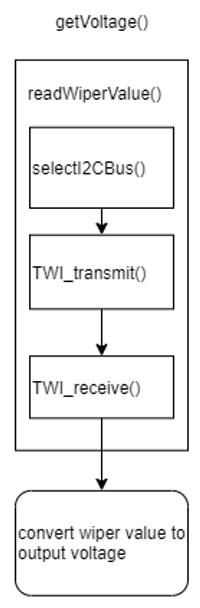
\includegraphics[scale=0.5]{software_getVoltage_flow_chart.png}
    \caption{Flow chart of the getVoltage funcion.}
\end{figure}

\begin{figure}[h]
    \centering
    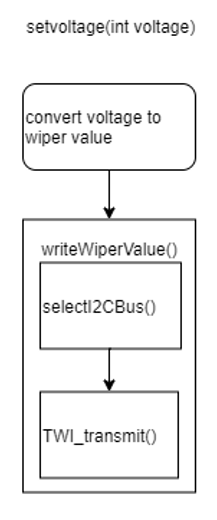
\includegraphics[scale=0.5]{software_setVoltage_flow_chart.png}
    \caption{Flow chart of the setVoltage funcion.}
\end{figure}

\begin{figure}[h]
    \centering
    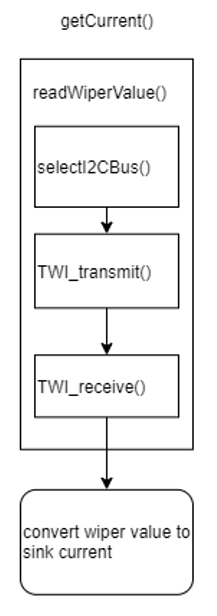
\includegraphics[scale=0.5]{software_getCurrent_flow_chart.png}
    \caption{Flow chart of the getCurrent funcion.}
\end{figure}

\begin{figure}[h]
    \centering
    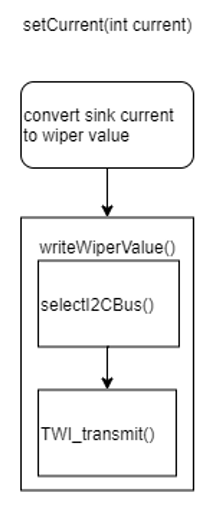
\includegraphics[scale=0.5]{software_setCurrent_flow_chart.png}
    \caption{Flow chart of the setCurrent funcion.}
\end{figure}


\subsection{Realization}
PCB text here.

\begin{figure}[h]
    \centering
    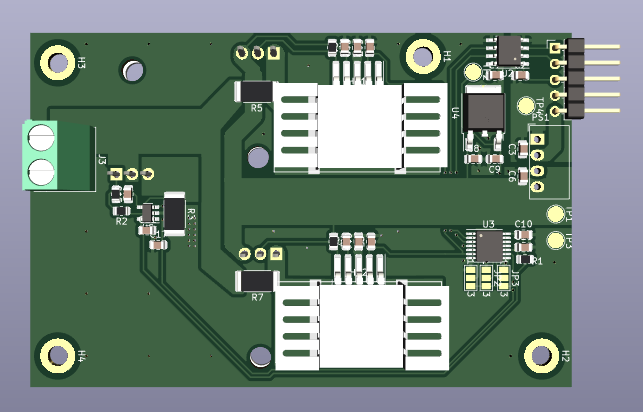
\includegraphics[scale=0.5]{pcb_cell_board_top.png}
    \caption{PCB layout of the top of the cell board.}
\end{figure}

\begin{figure}[h]
    \centering
    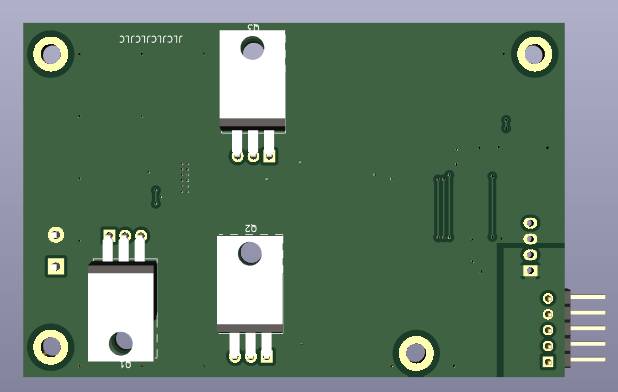
\includegraphics[scale=0.5]{pcb_cell_board_bottom.png}
    \caption{PCB layout of the bottom of the cell board.}
\end{figure}

\begin{figure}[h]
    \centering
    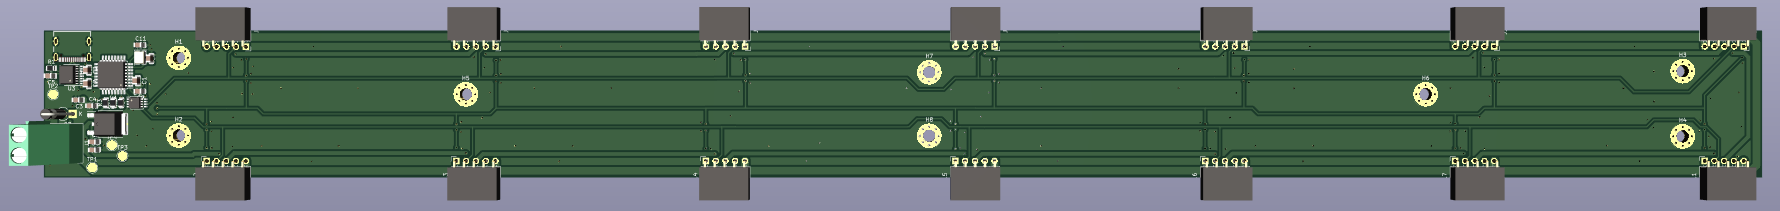
\includegraphics[scale=0.27]{pcb_model_board_top.png}
    \caption{PCB layout of the model board.}
\end{figure}

\subsection{Testing}
Testing text here.